\chapter{Geothermal Exploration with Machine Learning}\label{ch3:expl_ml_prep}
\section{Data Sources}\label{ch3:expl_data_src}
This investigation brings together a total of twenty-five (25) data sets covering the Southwestern NM study area. Data were collected from previously published works, open-access databases, or derived from those original sources as secondary products. The form of the data varies between pre-gridded raster files, point data sets with repeat or overlapping measurements, non-overlapping point sets, and line data. Previous researchers created raster files or raster-ready gridded data for ten of the features. Three features are generated by running procedures on one of the rasters. The remaining layers were created from polylines (5), overlapping points (4), and non-overlapping points (3). Although complex interactions between earth systems should be expected, these layers represent the ``independent'' or \textit{predictor} variables for analysis purposes. Section \ref{ch3:feat_corr} explains how evaluating collinearities between features allows for pre-screening before modeling, and further analysis of feature importances in Chapter \ref{ch5:expl_ml} helps hone in on the most influential features for simpler prediction models.

\begin{table}
\centering
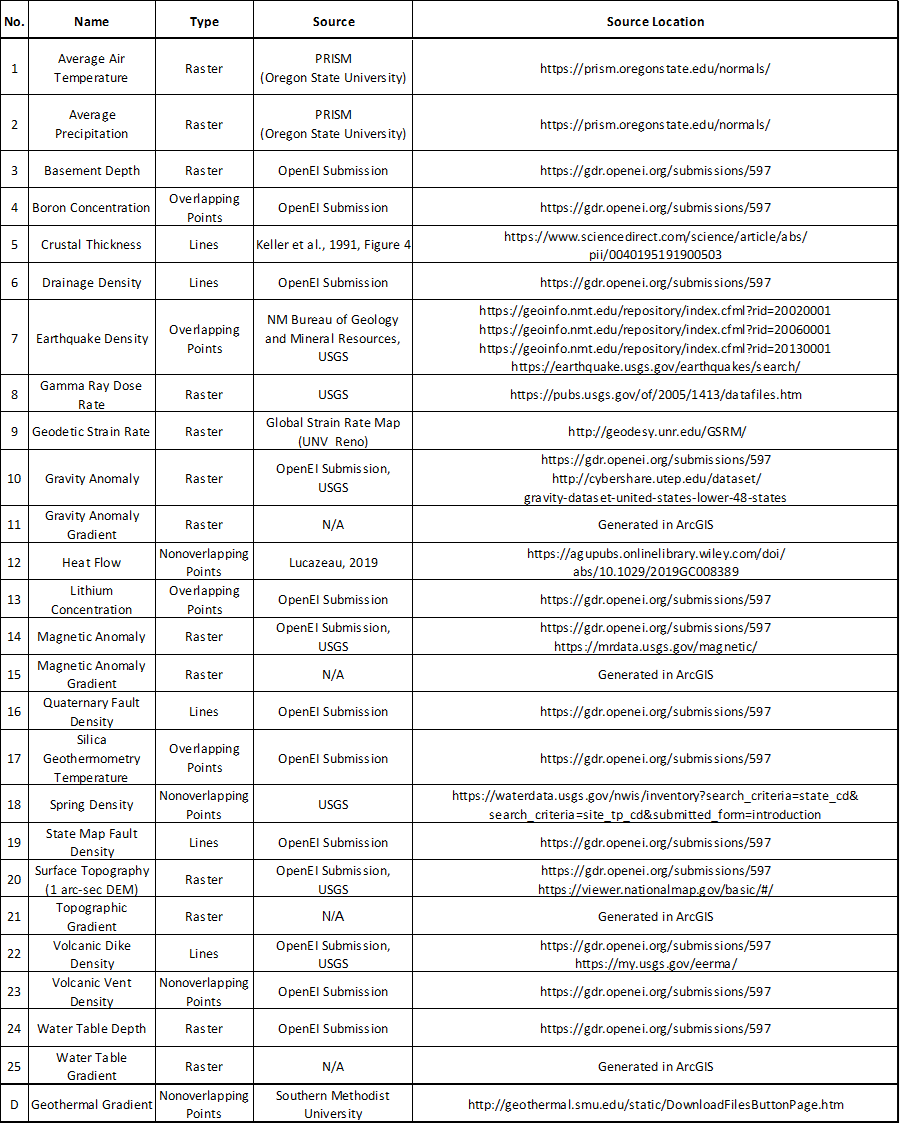
\includegraphics[width=\textwidth]{Table-Features.png}
\caption[Southwestern New Mexico feature list]{List of data sets included in this analysis. Data type, source, and source location are noted. Suggested feature-sensitive risk elements include fluids (F), heat/temperature (T), and structure/permeability (P). Numbered features are treated as predictor variables. `D' indicates the dependent or response variable. See Appendix \ref{app:A_data_layers} for details on how each feature GIS layer was constructed for modeling.}
\label{tab:features}
\end{table}

As discussed in Section \ref{ch2:sysfund}, viable geothermal systems require permeability, heat, fluids, seal, and recharge. Following the more simplified PFA risk elements of \citet{bielicki_hydrogeolgic_2015}, an explorationist will want to identify where fluids, heat, and permeability together define a favorable setting for a geothermal prospect. The chosen feature inputs collectively address all three elements, as noted in Table \ref{tab:features}. Rather than defining a ``dependent'' or \textit{response} variable that describes a total favorability score, this thesis focuses on a proof-of-concept predictive workflow for a physically-measurable quantity associated with the heat risk element: geothermal gradient. This choice was made because a) geothermal gradient provides a direct proxy for accessible heat content, b) gradient point data is available from suitable compilations of well measurements collected across the study area, and c) for EGS applications, the only risk element that must be naturally present is heat. Heat flow might be a reasonable alternative response variable, however heat flow values in the available well database were derived directly from geothermal gradient and hence are not primary source data. Geothermometer measurements (see Section \ref{ch2:geologic_data}) also suggest resource temperatures, but the uncertainty in fluid pathways leading to the sample location means these values suffer from less spatial and depth certainty than geothermal gradient.

Regarding the remaining two risk elements: permeability (i.e., results of wireline or core analysis) or fluids (i.e., flow test measurements) could be separately predicted using the same methods described in this study. A final favorability score, which is less straight-forward to calibrate for model validation and verification then geothermal gradient, could then be derived from the combined heat, permeability, and fluid probability maps as is done in PFA risk assessments. This suggestion is outside the scope of this thesis and thus appears in the list of future work opportunities (see Chapter \ref{ch9:future_work}).

Data loading, conditioning, modeling, and analysis were all conducted using a combination of ArcGIS Pro software and custom Python scripts. Final versions of the Python code are stored in GitHub and can be executed using Google Colab.
\vfill

\section{Data Preparation}\label{ch3:data_prep}
In order to experiment with a variety of machine learning methods, all input data sets must first be transformed into fully-complete \acrlong{gis} (\acrshort{gis}) layers such that any location within the study area has a corresponding set of predictor values. Steps taken to condition and process each layer are introduced in this chapter and detailed in Appendix \ref{app:A_data_layers}. The following section reviews several fundamental concepts and algorithms utilized in the preparation of the data layers.

\subsection{Fundamentals}\label{ch3:data_prep_fundamentals}
\subsubsection{Extents}\label{ch3:extents}
The data sets imported into ArcGIS and Python scripts for feature preparation required cropping, gridding, or, less frequently, extrapolation to match each other in coverage of the southwestern New Mexico study area. Two polygons were used for this purpose:

\begin{itemize}
\item \textbf{Regional Polygon}: this is a simple rectangular polygon capturing the broader southwestern NM region, defined by the following corner points in $^\circ$N Latitude and $^\circ$E Longitude: \\ (-31.3, -109.1), (31.3, -105.9), (35.4, -105.9), (31.3, -109.1)
\item \textbf{\acrlong{aoi} (\acrshort{aoi})}: this polygon appears in most map figures in this thesis and is the perimeter of a nine-county block in Southwest New Mexico that includes Cibola, Valencia, Catron, Socorro, Grant, Sierra, Luna, Dona Ana, and Hidalgo counties.
\end{itemize}

\subsubsection{Subsampling}
\label{ch3:fishnet}

Machine learning models generally treat data as a matrix of observations. The concept of a geospatial dataframe follows this paradigm, where each row represents a discrete location specified in latitude and longitude columns, and all other columns contain feature values for that location. Since the area outlined by the study AOI covers 97,469 km$^2$, and each location is described by 25 features and 2 map coordinates, the matrix of the study area at 1 km$^2$ resolution would be over 2.6 million values in size! This could be problematic since the time complexity of some machine learning methods shows non-linear growth with data size, e.g., decision trees (Section \ref{ch5:decision_trees}) have $O(\text{m} \cdot \text{n} \cdot log_2(\text{n}))$ complexity, where n is the number of observations and m is the number of features \citep{sani_computational_2018}. As such, a coarser resolution of $0.025^\circ$ ($\approx$2.5 km on average across the AOI) was selected as a manageable subsampling interval for this study. To accomplish this, the ArcGIS \textit{Create Fishnet} tool was used to generate a $0.025^\circ$ x $0.025^\circ$ mesh that, when constrained to the AOI polygon, consists of 15,137 point locations (Figure \ref{fig:fishnet}). Data preparation steps use this fishnet point set where noted in Appendix \ref{app:A_data_layers}, and final model predictions are made on these points to enable direct comparison between different model results. 

\begin{figure}
\centering
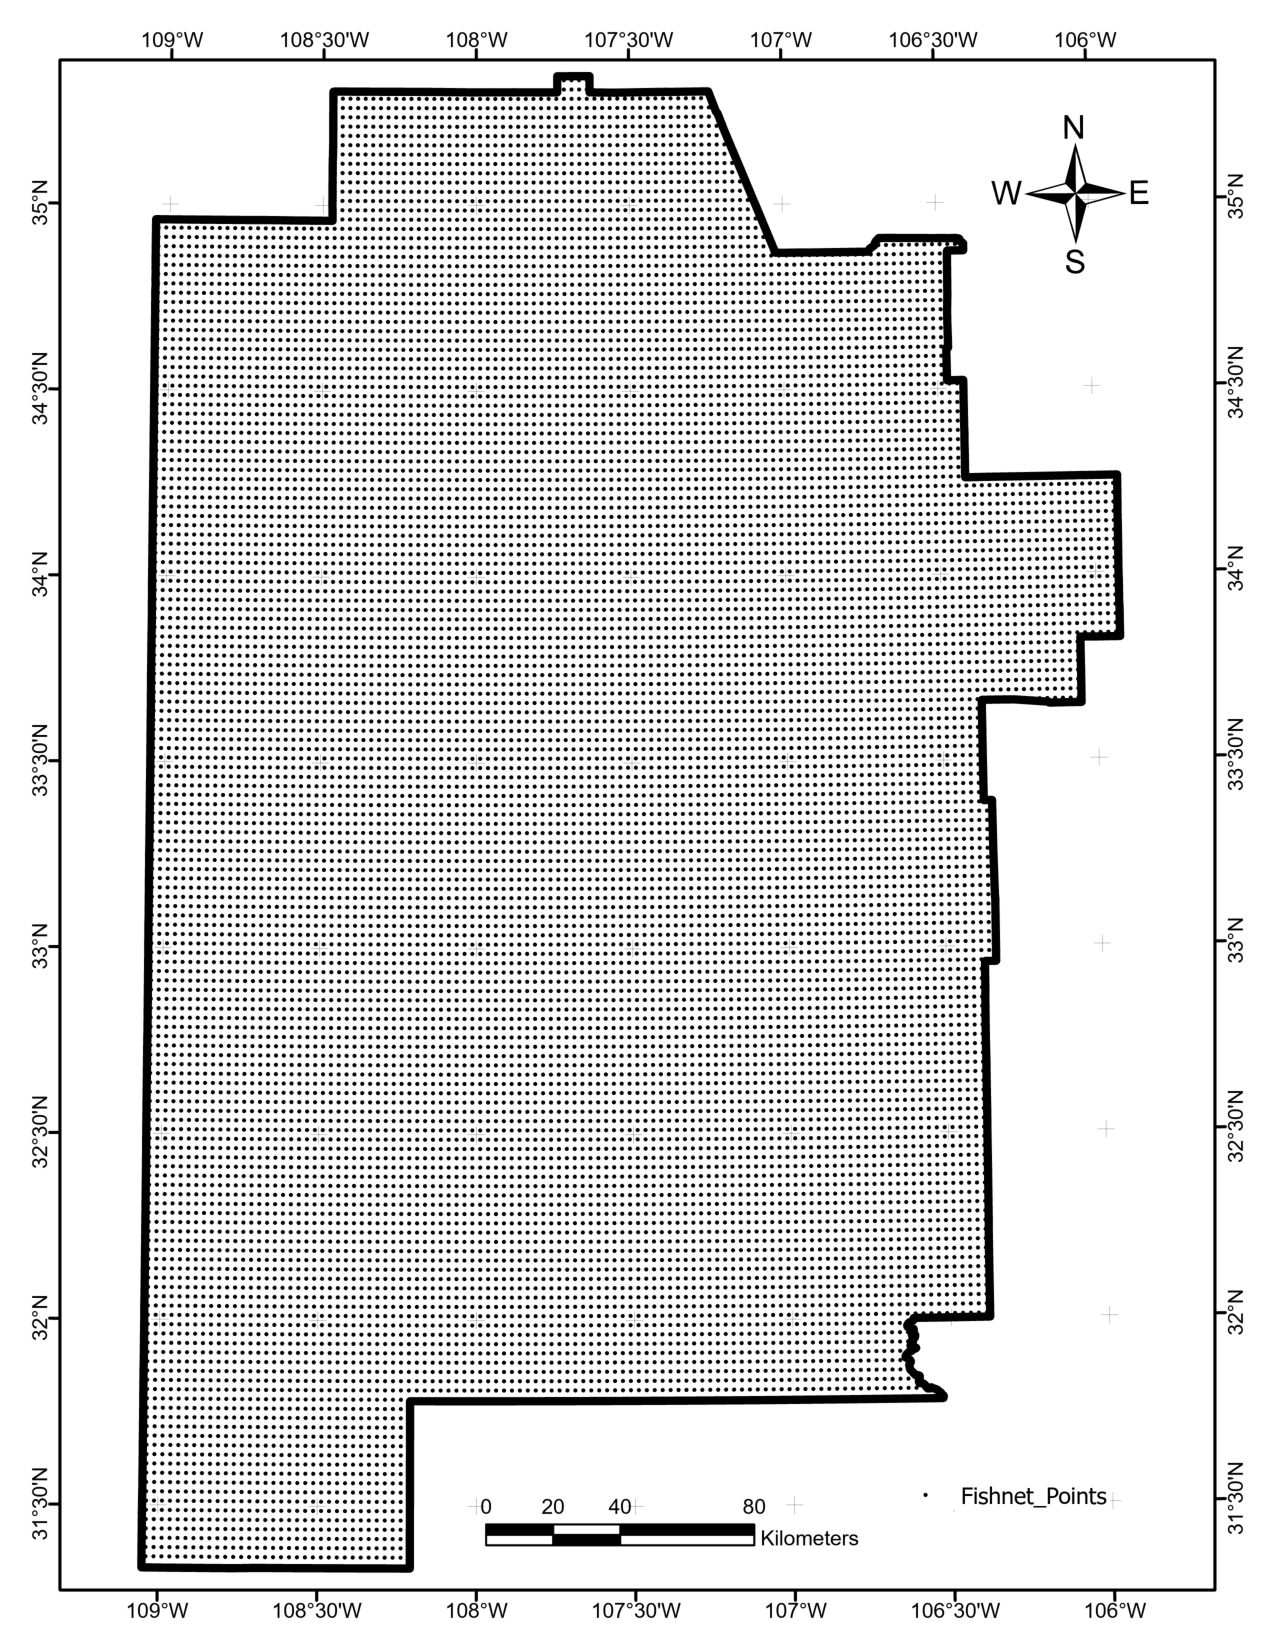
\includegraphics[width=0.75\linewidth]{templates/images/Figure-Fishnet.pdf}
\caption[Fishnet point set]{Fishnet of points spaced $0.025^\circ$ apart in latitude and longitude. The fishnet point set is used for data preparation and model predictions.} 
\label{fig:fishnet}
\end{figure}

\subsubsection{Density Estimation}\label{ch3:density_est}
One technique for converting a discrete set of points into a continuous field of values uses the concept of point density. The \acrlong{kde} (\acrshort{kde}) method fits a smooth function (kernel) to each point with the constraint that the volume under a kernel surface is 1.0. Density values assigned to cells of a gridded surface or raster image represent the sum over the kernels crossing those cells. The kernel density tool can provide an estimate of density anywhere within the AOI, but it requires a kernel radius that sets the distance over which a point influences the density value. If left undefined, ArcGIS defaults to an optimal radius value based on a bandwidth formula \citep{esri_kernel_2021}. ArcGIS uses Silverman quartic kernel as the functional basis in the \textit{Kernel Density} operation \citep{esri_kernel_2021,silverman_density_1986}.

Polyline data can also be fit with smoothly-curved surfaces using the density concept. The maximum value of the elongate surface follows the trace of the polyline, and the surfaces decays in value away from the line over a distance determined by the radius, which defaults to the bandwidth estimate. The volume under the surface scales with line length. For more details on the ArcGIS implementation, refer to the \textit{Density toolset} documentation on \textit{Kernel Density} \citep{esri_kernel_2021}.

\subsubsection{Surface Fitting}\label{ch3:surface_fit}
A multitude of algorithms exist for the purpose of fitting a set of values with a surface, thereby providing a means for interpolating missing values. Methods used in this thesis include the following four operations:

\begin{itemize}
\item{\textbf{Splines}}\label{ch3:splines} - Spline functions have a well-defined mathematical formulation that minimizes curvature while exactly fitting the input points. Regularized splines add a third derivative term, controlled by a weight parameter, that enforces a higher degree of smoothness with the trade-off of some misfit of the input data. This is helpful if outliers in the input point set would otherwise distort the spline fit. For details on the ArcGIS implementation, refer to the \textit{Interpolation toolset} documentation on the \textit{Spline} function \citep{esri_spline_2021}.
\item{\textbf{Topo to Raster}}\label{ch3:topo2r} - The ArcGIS \textit{Topo to Raster} operation creates surfaces that honor the input data, typically contour sets, while ensuring i) correct representation of abrupt morphological features like rivers and ridges and ii) connectedness of drainage patterns. Specifically, \textit{Topo to Raster} uses an iterative finite difference method and an algorithm to remove sink points not supported by the input data, assuming natural sinks are rare and erroneous features in an interpolated surface. For details on the ArcGIS implementation, refer to the \textit{Interpolation toolset} documentation on the \textit{Topo to Raster} function \citep{esri_topo_2021}.
\item{\textbf{Ordinary Kriging}}\label{ch3:kriging} - Kriging methods are geostatistical algorithms that take the correlation distance and directional bias into account when creating a surface. The two tasks involved in kriging include first estimating the functions that characterize these spatial relationships, then using these functions to generate predictions for interpolation (and extrapolation). For the first task, semivariograms are calculated by binning the semivariance of points based their distance from each other, then fitting a model curve (e.g. linear, spherical, exponential) to these values. Semivariograms can be anisotropic, meaning they can vary with direction. The second task uses the semivariogram to define a weighted average of the input data when estimating new values. For more details on the ArcGIS implementation, refer to the \textit{Interpolation toolset} documentation on the \textit{Kriging} function \citep{esri_kriging_2021}.
\item{\textbf{\acrlong{ebk} (\acrshort{ebk})}}\label{ch3:ebk} - The EBK algorithm extends ordinary kriging by automating parameter selections and accounting for uncertainty in semivariogram estimation. Ordinary kriging generates a single variogram and treats it as ground truth while EBK generates an ensemble of semivariograms that can more accurately estimate standard errors. As a computationally heavy methodology, EBK takes much longer to apply than other methods. For more details on the ArcGIS implementation, refer to the documentation on the \textit{Empirical Bayes Kriging} function \citep{esri_empirical_2021}.
\end{itemize}

\subsection{Data Conditioning}\label{ch3:conditioning}
\begin{wrapfigure}{R}{0.35\linewidth}
\centering
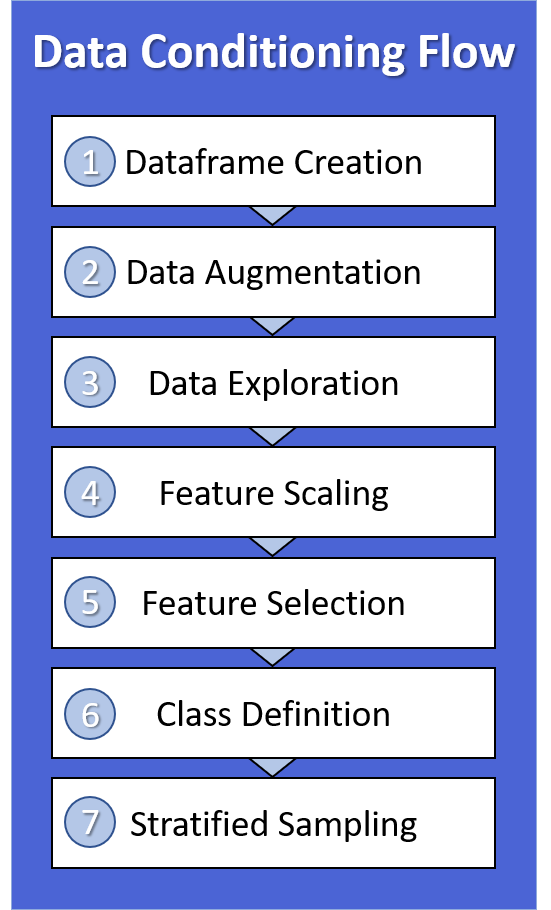
\includegraphics[width=0.89\linewidth]{templates/images/Flow-DataConditioning.png}
\singlespacing
\caption[Data conditioning workflow]{Workflow for conditioning data prior to predictive modeling.}
\label{fig:DC_Flow}
\end{wrapfigure}
After collecting the various data layers, several data conditioning steps were taken in order to explore variable relationships, rationalize feature choices, and prepare data values for modeling. Figure \ref{fig:DC_Flow} outlines the general workflow followed, detailed more extensively below.

\subsubsection{Dataframe Creation}
Feature GIS maps spanning the full AOI provide the primary resource for a data set, but predictions of geothermal gradient require ground truth observations for training a predictive model. Initially, two separate data sets could be constructed for further evaluation. The first is a \acrlong{fds} (\acrshort{fds}) that includes of a fishnet extraction of the feature values (Figure \ref{fig:fishnet}), resulting in 15,137 records for the 25 predictors. This data set does not include values for the response variable. The geothermal gradient layer described in Section \ref{app:dl_geothermal_gradient} is a derived layer useful for comparison, but not ground truth. The second data set was built from actual geothermal gradient observations in the SMU data set, combined with 25 feature values extracted from the GIS maps at the observation locations. This data set is hereafter referred to as \acrlong{wds} (\acrshort{wds}). Both FDS and WDS were stored in ``geodataframes'' consisting of the feature values and their associated latitude and longitude coordinates. These structured matrices are compatible with machine learning techniques like those found in the scikit-learn \citep{pedregosa_scikit-learn_2011} and TensorFlow \citep{abadi_tensorflow_2016} Python packages. 

\subsubsection{Data Augmentation}
\label{ch3:augmentation}

\begin{wrapfigure}{R}{0.5\linewidth}
\centering
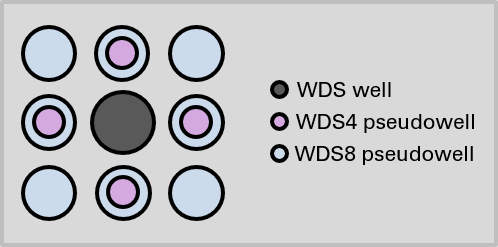
\includegraphics[scale=0.9]{templates/images/Figure-AugmentedWells.png}
\singlespacing
\caption[Data augmentation strategy]{The data augmentation strategy creates neighboring well locations around each original well in the WDS (dark gray). For WDS4, pseudowells (purple) are placed to the N, S, E, and W. For WDS8, pseudowells (blue) are placed at eight locations around the central well. Latitude and longitude offsets are $\pm0.01^\circ$ for pseudowell placement.}
\label{fig:data_augmentation}
\end{wrapfigure}

Noting the AOI under investigation spans over 97,000 km$^2$, the relatively small size of WDS raises concern over whether enough data is available to obtain data-driven insights using supervised learning methods. If predictions are reduced to just locations within the fishnet point set, there are still 2 orders of magnitude difference between ground truth observations and the points being predicted, exacerbated further by the need to partition the input data into one subset for training and two others for model validation and testing as a machine learning best practice \citep[e.g.,][p.\ 222]{hastie_elements_2009} (see Section \ref{ch3:strat_sample}). 

Data augmentation methods boost the size of a sparse data set by using basic assumptions or heuristics to create additional data points. This study applies the concept of spatial autocorrelation at the heart of variography and kriging methods; in geography, all things are related, but the correlation increases as the spatial distance decreases \citep[Chapter\ 13]{gimond_intro_2021}. For each well location in the WDS, an additional four points were placed to the north, south, east, and west by adding or subtracting a constant 0.01$^\circ$ for each well’s geographic coordinates (Figure \ref{fig:data_augmentation}). Feature values were extracted from the layer maps in ArcGIS at these ``pseudowell'' locations. For the response variable, geothermal gradient, an interpolation layer was created using the ArcGIS \textit{Kriging} function with spherical variogram, auto-determined lag size of 0.097, and variable search radius with 12-point requirement. Gradient values were extracted from this layer for each pseudowell. The use of an interpolated gradient layer avoided conflict in pseudowell values for close-proximity real well locations since step-out pseudowells for neighboring original wells could (and do) overlap. This overall workflow generated a new data set with 2,995 observations within the study AOI, referred to as \acrshort{wds4}. 

Extending this method further, a second augmented data set placed pseudowells to the NE, SE, NW, and SW as well, resulting in eight pseudowells for every original well in the WDS (Figure \ref{fig:data_augmentation}). Restricting the results to the AOI, this produced a data set with 5,386 observations (\acrshort{wds8}) for use in training and testing of machine learning models.

\subsubsection{Data Exploration}
The comprehensive coverage of FDS makes it an appealing data set to use for exploring the attributes and relationships of the 25 data layers. Although care was taken to ensure each GIS layer fully spanned the AOI, a search for missing values identified 163 \acrshort{nan}s (not a number, i.e., unassigned values) among the features. The corresponding data rows plot along the study area boundary and likely represent places where one or more data layers ended just short of the fishnet point locations. These rows were dropped from FDS, reducing its size to 15,007 records.

Histograms can offer insights on the data distributions of predictor variables. Based on Figure \ref{fig:unscaled_hists}, only the magnetic anomaly layer has the appearance of a zero-mean Gaussian distribution. All other variables are offset and skewed to some extent. Many statistical tools rely on the assumption of normally-distributed random variables, so skewness can be problematic for modeling \citep[p.\ 85]{montgomery_statistical_2012}. These results suggest variable scaling and transformations will be a useful part of data preparation \citep[p.\ 221]{montgomery_statistical_2012}. 

\begin{figure}[!htp]
\centering
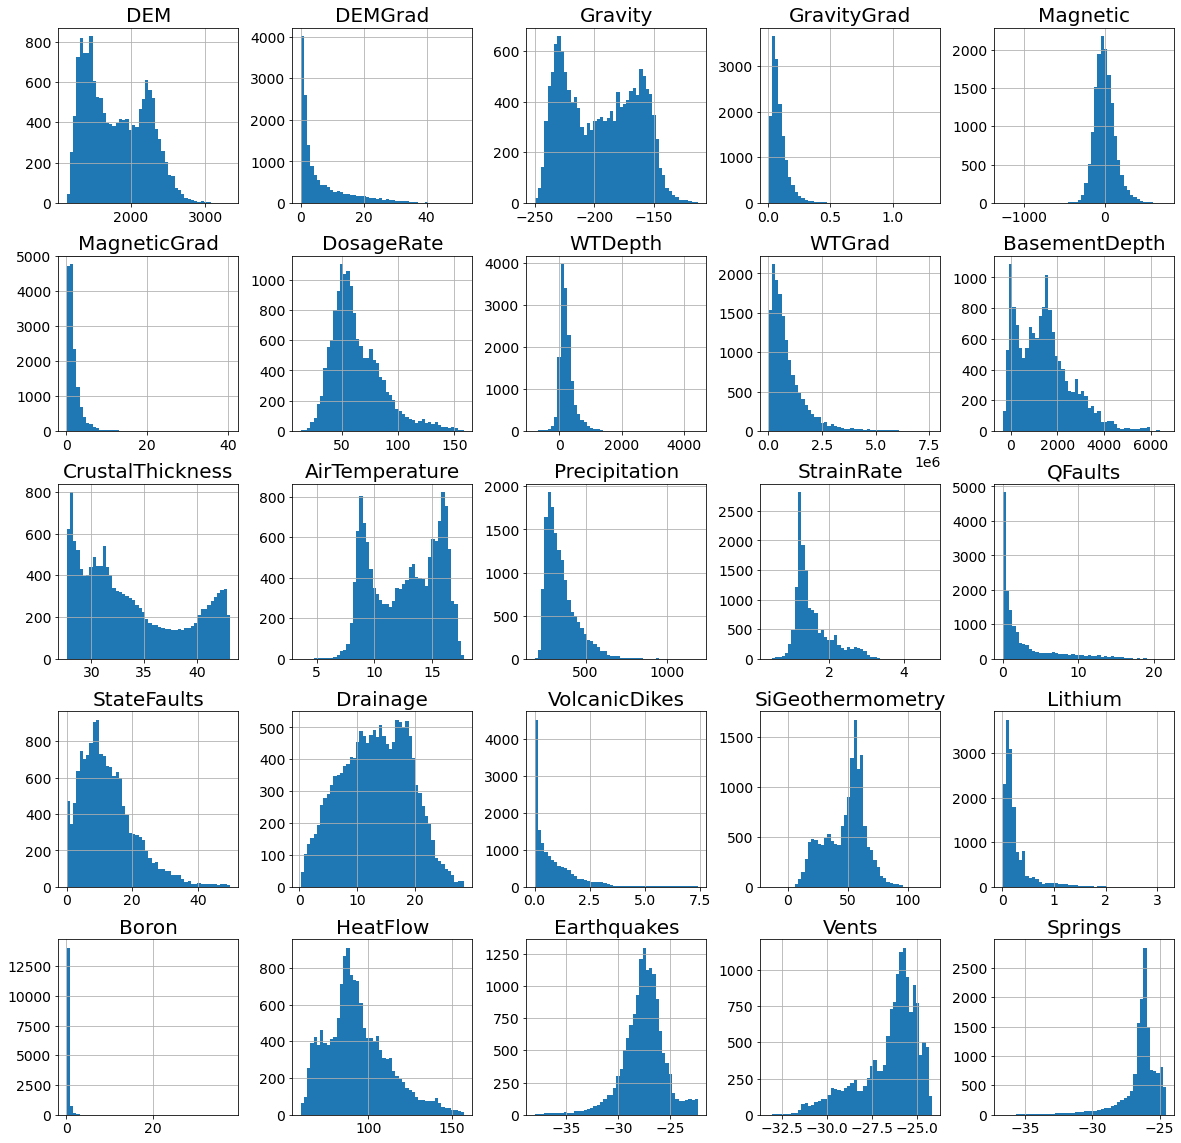
\includegraphics[width=\textwidth]{templates/images/Figure-Unscaled_Histograms.png}
\caption[Unconditioned FDS histograms]{Histograms of the 25 features using 50 bins and FDS data. No scaling or transformations were applied to the data.}
\label{fig:unscaled_hists}
\end{figure}

Scatter plots between variables can highlight collinear behavior where a close relationship between two predictors creates uncertainty in their balance, that is, their individual contributions to the response variable \citep[p.\ 99]{james_introduction_2013}. This can reduce the accuracy of model parameters like regression coefficients, impact the statistical significance of predictors, and lead to overly complex models \citep[p.\ 100-101]{james_introduction_2013}. Figure \ref{fig:unscaled_scatter} illustrates all permutations of feature pairwise relationships. Although individual plots are too small to appreciate in detail, the overall shapes of the plots suggests some linear behavior between a handful of variables. The inset maps illustrate two examples of collinearity, and the third shows how skewness in variable distributions makes it difficult to discern some feature relationships.

\begin{figure}[!htp]
\centering
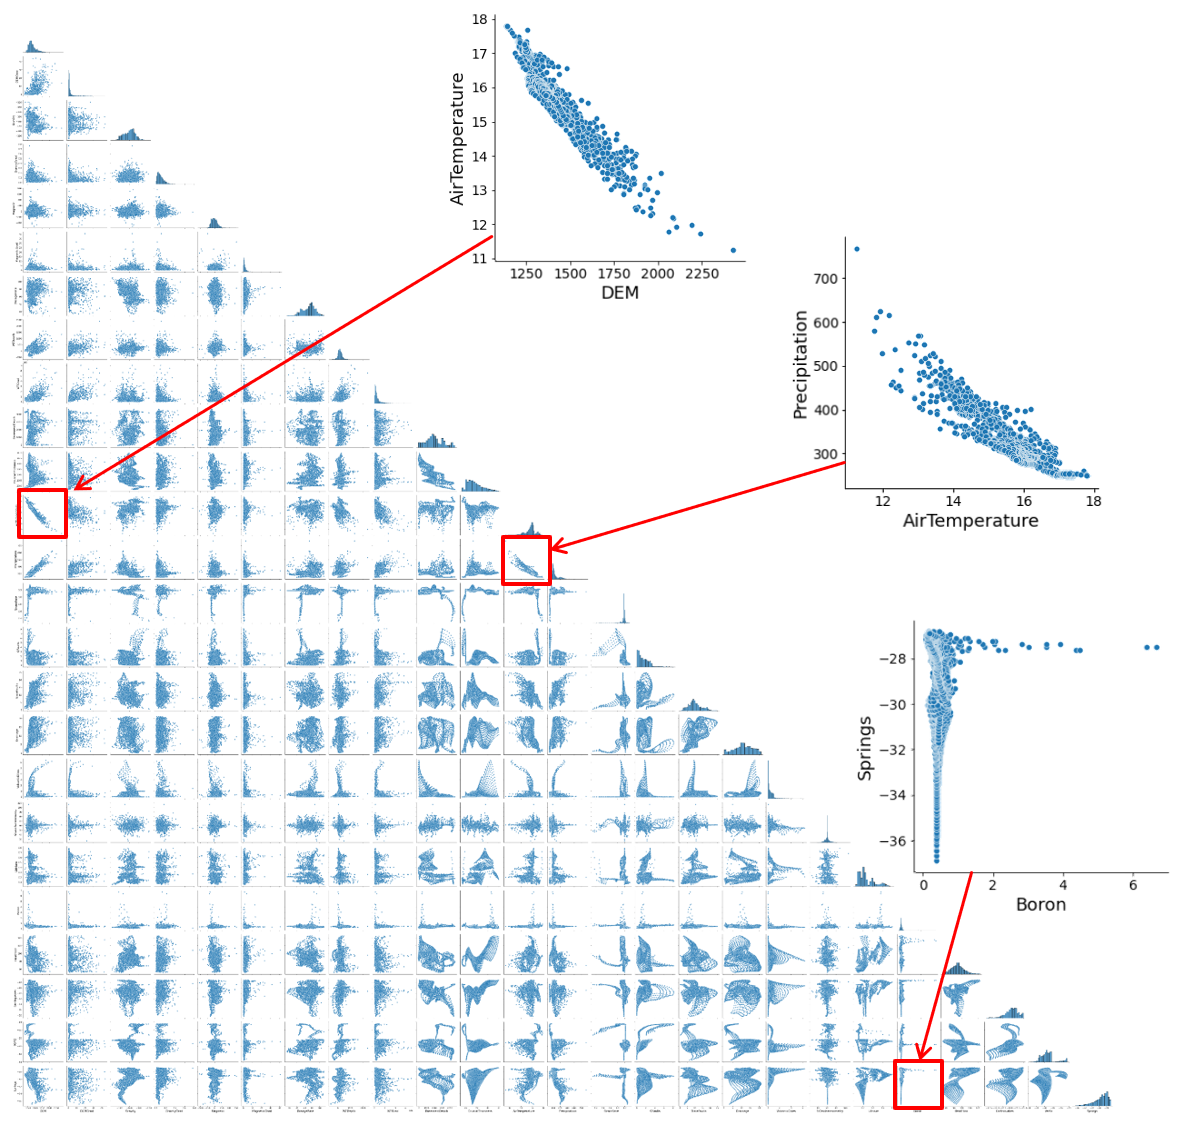
\includegraphics[width=\textwidth]{templates/images/Figure-Scatterplot_Unscaled_Features.png}
\caption[Unscaled FDS scatter plots]{Scatter plots between all possible pairs of the 25 features. The upper two plot call-outs illustrate collinear relationships. The lowermost highlighted plot shows the impact of skewed distributions. Note the difference in axis ranges depending on the variable. All plots show the first 2,000 points of the 15,007-point FDS.}
\label{fig:unscaled_scatter}
\end{figure}

\subsubsection{Feature Scaling}\label{ch3:scaling}
Large differences in the ranges and average values of the predictor variables are also evident in the scatter plots in Figure \ref{fig:unscaled_scatter}. For some machine learning algorithms, variables with larger value ranges can have an out-sized effect on the model, so scaling variables to comparable ranges and removing variable bias is an important step in data conditioning. Scaling also makes a predictor closer to the standard normal in appearance, i.e., $N(\mu=0, \sigma=1)$, as implicitly required by some statistical methods. The scikit-learn \textit{StandardScalar} function transforms data using the Z-score formulation \citep{scikit-learn_sklearnpreprocessingstandardscaler_2021}:

\begin{equation}
    Z = \frac{(x - \mu)}{\sigma}
\end{equation}

This data scaling can be directly paired with non-linear data transformations that alter the shape of variable distributions, replacing skewness with more Gaussian-like symmetry. One such transformation is the Yeo-Johnson method, which can handle both positive and negative data. The Yeo-Johnson power transformation actually represents a family of transformations, the choice of which depends on a single parameter, $\lambda$ \citep{yeo_new_2000}:

\begin{equation}
    x_i^{(\lambda)} = 
    \begin{cases}
      [(x_i + 1)^{\lambda)}-1]/\lambda & \text{if $\lambda \neq 0$, $x_i \geq 0$,}\\
      \ln{(x_i + 1)} & \text{if $\lambda = 0$, $x_i \geq 0$,}\\
      -[(-x_i + 1)^{2-\lambda}-1]/(2-\lambda) & \text{if $\lambda \neq 2$, $x_i < 0$,}\\
      -\ln{(-x_i + 1)} & \text{if $\lambda = 2$, $x_i < 0$}
    \end{cases}  
\end{equation}

Scikit-learn supports Yeo-Johnson through the \textit{PowerTransformer} preprocessing tool that automatically estimates the $\lambda$ parameter using maximum likelihood \citep{scikit-learn_sklearnpreprocessingpowertransformer_2021}. Figure \ref{fig:scaled_hist} shows the same histograms after applying both standard scaling and Yeo-Johnson transformation to the predictor variables. Many of the distributions appear much less skewed, and all have zero-mean and unit variance.

\begin{figure}[!htp]
\centering
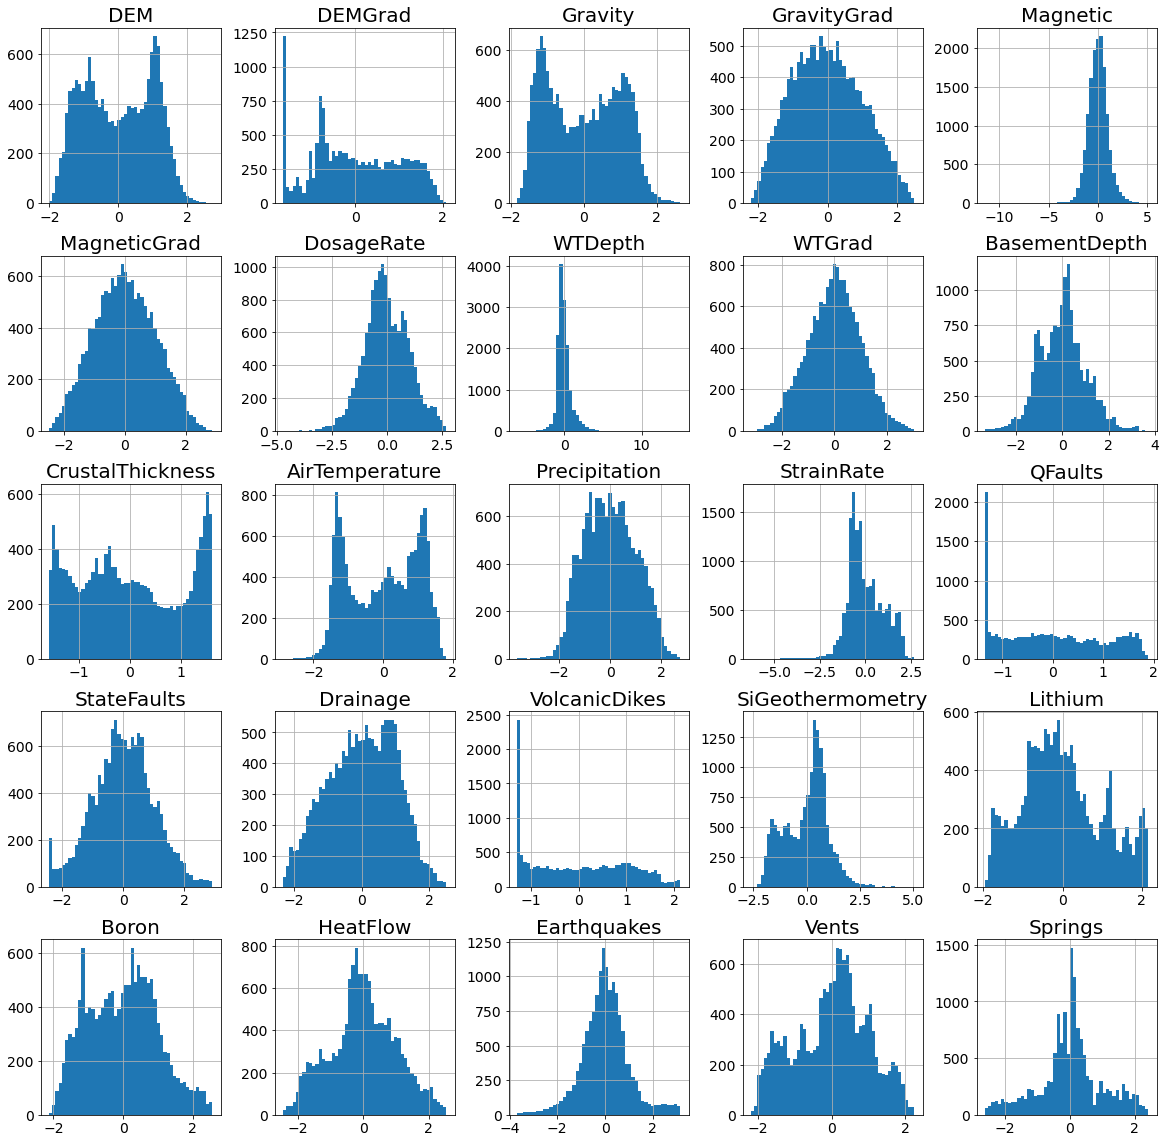
\includegraphics[width=\textwidth]{templates/images/Figure-Scaled_Histograms.png}
\caption[Conditioned FDS histograms]{Histograms of the 25 features after standard-scaling and Yeo-Johnson transformation of FDS. Plots use 50 bins.}
\label{fig:scaled_hist}
\end{figure}

Scaling and transformation also impacts the variable pairwise scatter plots. Figure \ref{fig:scaled_scatter} illustrates the improvement in scatter plot appearances as a result of the feature conditioning. With greater spread in the variable distributions, relationships are more readily apparent.

\begin{figure}[!htp]
\centering
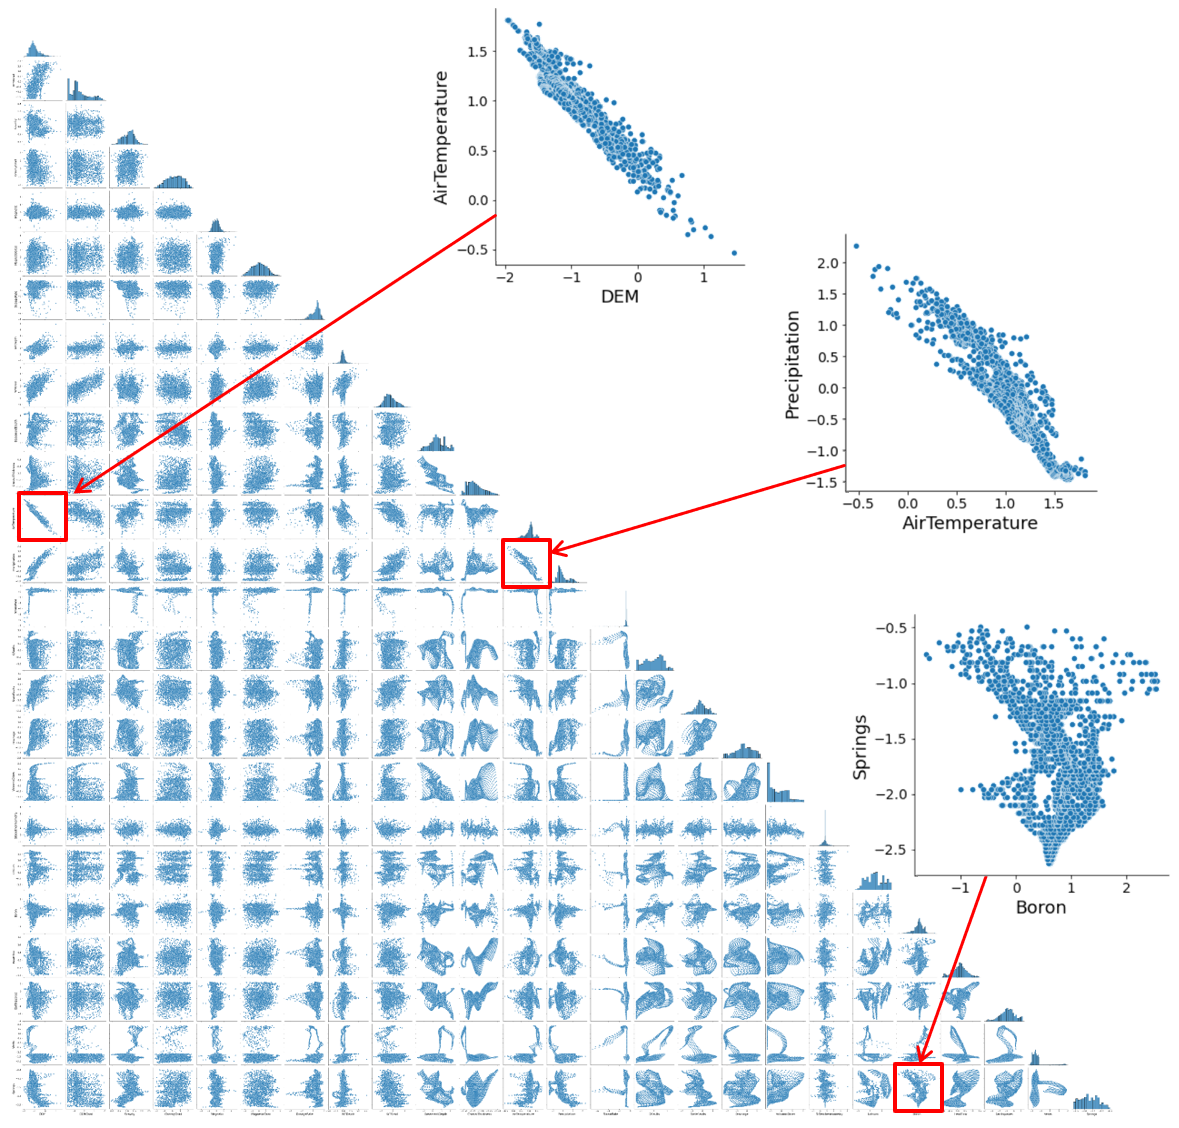
\includegraphics[width=\textwidth]{templates/images/Figure-Scatterplot_Scaled_Features.png}
\caption[Scaled FDS scatter plots]{Scatter plots between all possible pairs of the 25 features after standard scaling and Yeo-Johnson transformation for FDS. The upper two plot call-outs illustrate collinear relationships. The lowermost highlighted plot shows the impact of Yeo-Johnson transformation on revealing variable relationships that were hidden by skewed distributions. All plots show the first 2,000 points of the 15,007-point FDS.}
\label{fig:scaled_scatter}
\end{figure}

\subsubsection{Feature Correlation}\label{ch3:feat_corr}
Another way to evaluate collinearity between two features is to calculate their correlation coefficient. The standard Pearson correlation coefficient ($r$) is strictly defined as the covariance between two variables, scaled by the product of their standard deviations. On a per-sample basis, this becomes \citep[p.\ 70]{james_introduction_2013}:

\begin{equation}
    r = \frac{\Sigma(x_i-\bar{x})(y_i-\bar{y})}{\sqrt{\Sigma{(x_i-\bar{x})^2} \Sigma{(y_i-\bar{y})^2}}}
\end{equation}

When $r$ is close to zero, no measurable covariance takes place between the two variables. Values close to 1 or -1 suggest the two variables are linearly-related, where the sign indicates direction of the relationship. A lower triangular matrix of pairwise correlation coefficients was calculated using the scaled, transformed version of FDS (Figure \ref{fig:corr_matrix}). Average Air Temperature stands out as highly collinear with multiple variables: DEM (-0.97), Gravity Anomaly (0.89), and Crustal Thickness (-0.89). Crustal Thickness also shows some collinearity with Gravity Anomaly (-0.88) and DEM (0.80). The same is true for Gravity and DEM (-0.83).

\begin{figure}[!htp]
\centering
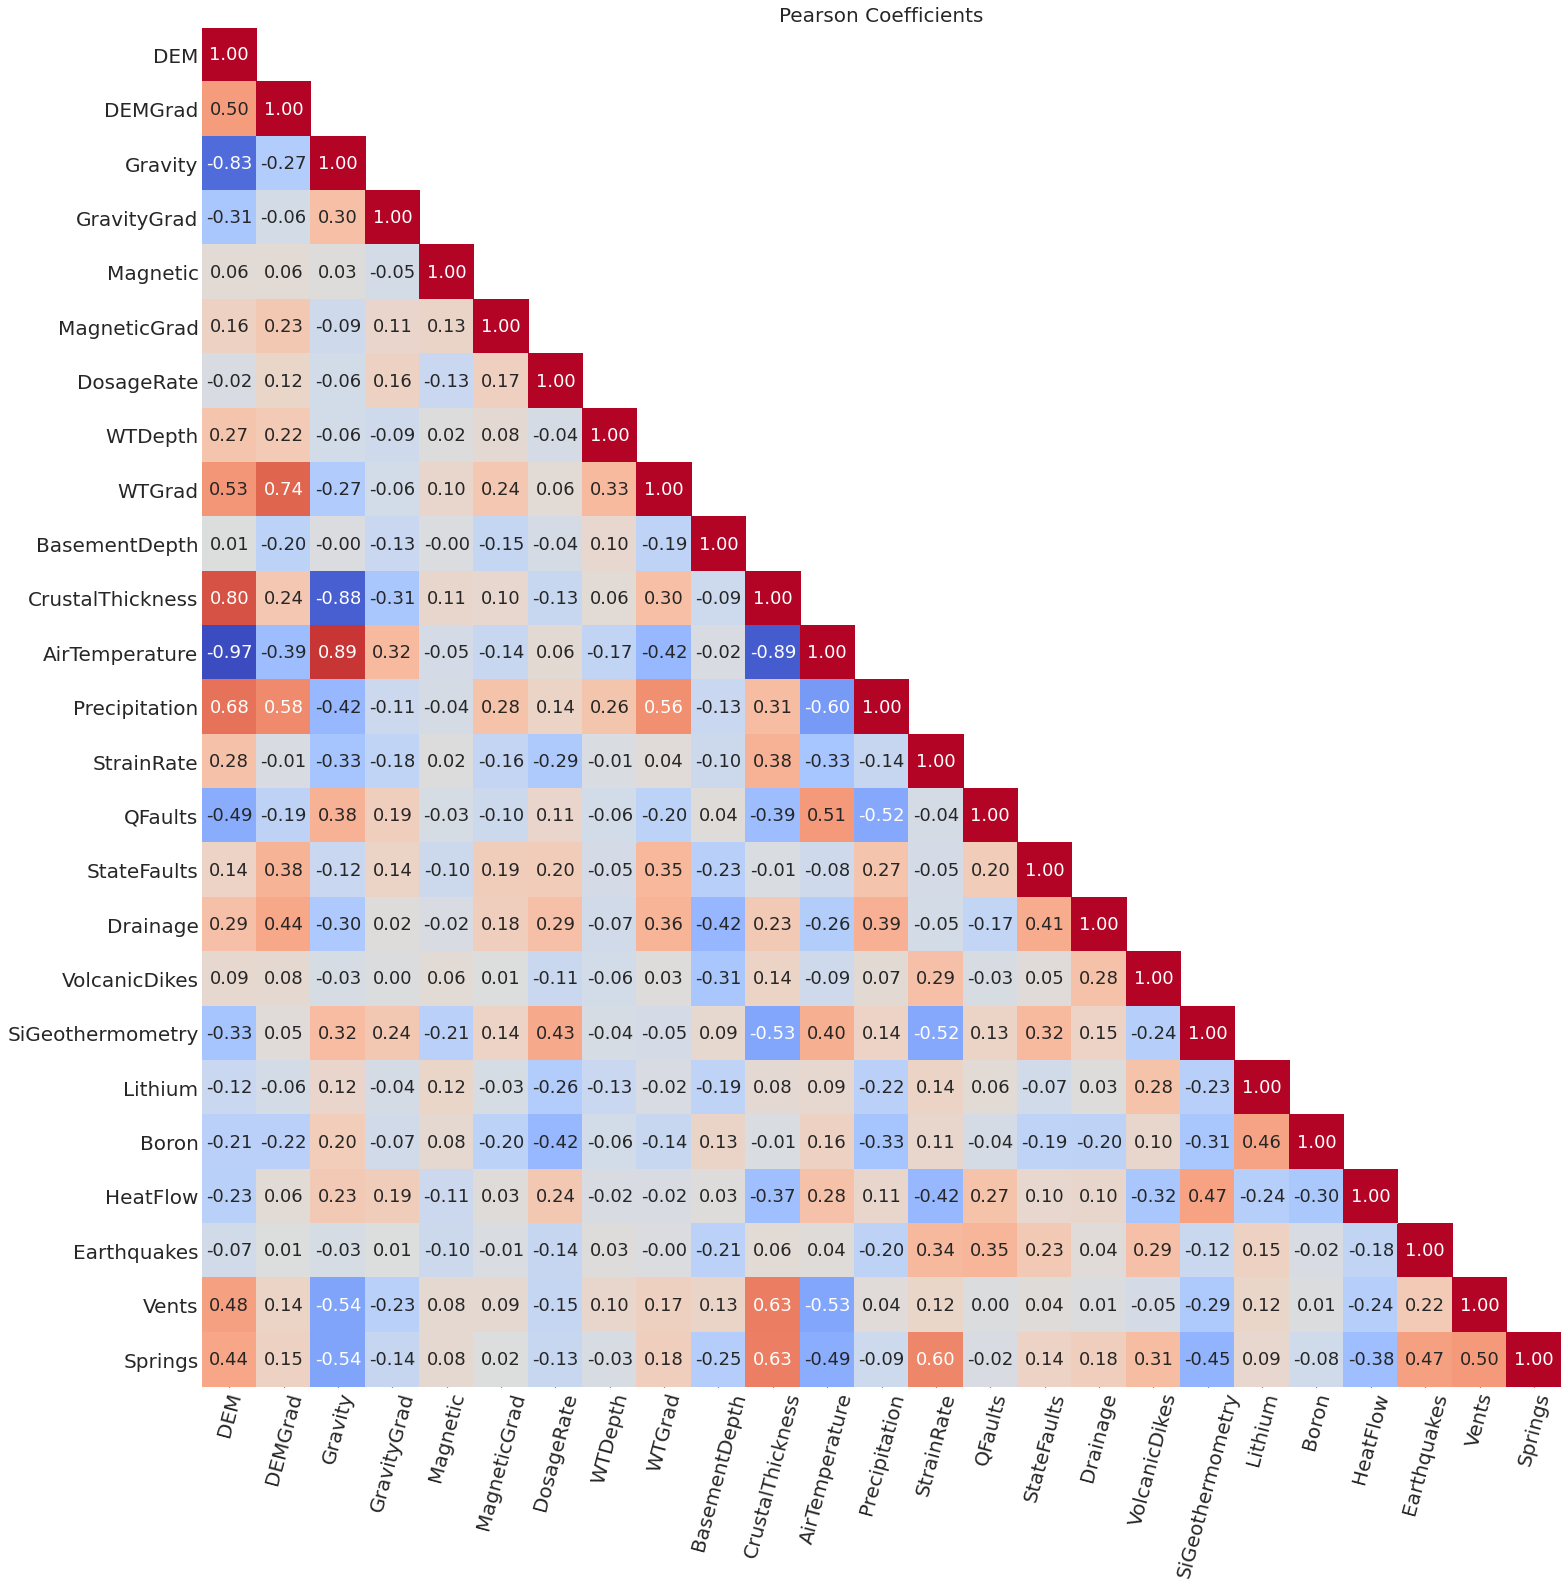
\includegraphics[width=\textwidth]{templates/images/Figure-Scaled_Correlation_Matrix.png}
\caption[Feature correlation matrix]{Correlation matrix with Pearson correlation scores for each feature pair based on the scaled and transformed version of the FDS.}
\label{fig:corr_matrix}
\end{figure}

Focusing on the related Earth systems, the logic behind these relationships makes sense. High surface elevations recorded in the DEM layer will have correspondingly lower average air temperatures, hence snow caps appearing on mountains. In addition, if the crust is assumed to be in isostatic equilibrium with the mantle --- like an iceberg floating in the ocean --- topographic highs will be supported by thick roots and DEM will directly covary with crustal thickness. And since crustal densities are less than those of the underlying mantle, displacement of upper mantle by crustal roots (high crustal thickness) results in a lower average density and negative gravity anomaly values. The reverse is true as well; thinner crust will correspondingly tie to positive gravity anomaly values.  

Of these variables, only Air Temperature and DEM have a correlation value over 0.9. In fact, a 0.97 $r$-value suggests Air Temperature and DEM are nearly interchangeable in the value of information they provide to a predictive model. Since air temperature does not directly relate to subsurface characteristics except for thermal conditions at zero-depth, Average Air Temperature can be removed from the main set of predictors to reduce overall collinearity in the data set. Crustal Thickness and Gravity Anomaly both similarly show non-ideal $r$-values, but feature ranking while modeling will provide another opportunity to consider which of them might need to be removed (e.g., Section \ref{ch5:xgb_shapley}).

\subsubsection{Classification Options}
\label{ch3:gradient_classes}

Geothermal gradient can be treated as a continuous variable and predicted directly using regression methods. Alternatively, binning the geothermal gradient into discrete ranges changes the approach into a classification problem. In the context of exploration, geospatial classifications have a direct corollary in the typical traffic-light coloration of PFA favorability maps and other simplified displays of complex risk. Furthermore, regression model results provide exact geothermal gradient estimates, which could easily be mistaken for certainty in a largely under-constrained problem. The binning approach is adopted in this thesis largely based on the work of previous researchers.

\begin{wraptable}{R}{0.4\linewidth}
\centering
\begin{tabular}{|c|c|}
\hline
\textbf{Gradient Range} & \textbf{Class} \\ \hline
{[}\;0 K/km, 30 K/km)     & 0                    \\ \hline
{[}\;30 K/km, 40 K/km)    & 1                    \\ \hline
{[}\;40 K/km, 60 K/km)    & 2                    \\ \hline
{[}\;60 K/km, 999 K/km)   & 3                    \\ \hline
\end{tabular}
\singlespacing
\caption[Geothermal gradient classes]{Geothermal gradient ranges and assigned class values using set notation. Ranges are left-inclusive.}
\label{tab:geothermal_gradient_classes}
\end{wraptable}

The \textit{Geothermal Gradient Map of the Conterminous United States} published in 1991 separates geothermal gradient into five 15 $^\circ$C/km bins that end with 60-75+ $^\circ$C/km \citep{lanl_geothermal_1991}. \citet{armstead_heat_1987} instead defined non-thermal gradients as 20-25 $^\circ$C/km, thermal gradients as $\leq$38 $^\circ$C/km, and hydrothermal gradients as 60-80 $^\circ$C/km on average. \citet{tester_economic_1990} reframed this model with representative values for three EGS grades: high = 80 $^\circ$C/km, mid = 50 $^\circ$C/km, and low = 30 $^\circ$C/km. In a later iteration, \citet{herzog_economic_1997} reasserted ranges for EGS resources: high-grade for >60 $^\circ$C/km, mid-grade for 40-60 $^\circ$C/km, and low-grade for <40 $^\circ$C/km. This thesis extends the Herzog model by adding a non-thermal range as <30 $^\circ$C/km, recognizing the average geothermal gradient ranges from 25-30 $^\circ$C/km and anything below that would be ill-suited for geothermal exploration and development (Table \ref{tab:geothermal_gradient_classes}).

Preparation of well data sets WDS, WDS4, and WDS8 first involved removing records with NaN values or negative geothermal gradients. The remaining records were split into the gradient categories in Table \ref{tab:geothermal_gradient_classes}. Distributions of class values for all data sets are shown in Table \ref{tab:data_set_class_count}. For FDS, the class break-down is based on the extrapolated \citet{bielicki_hydrogeolgic_2015} geothermal gradient layer (Figure \ref{fig:feat_pfa_geotherm_gradient}) sampled using the point fishnet (Figure \ref{fig:fishnet}). Note that class imbalance exists in all data sets; mid-grade values dominate in the FDS, but the well data sets show a bias toward high-grade examples with few non-thermal examples. This is a common conundrum when using well data for characterization and analysis; drilling campaigns tend to target areas to drill based on chance of success rather than drilling at random, so low-side under-representation tends to be ubiquitous. The topic of class imbalance is discussed again in \textbf{Section XX}.  

\begin{table}[htp]
\centering
\begin{tabular}{c|c|c|c|c|}
\cline{2-5}
                              & FDS    & WDS & WDS4  & WDS8  \\ \hline
\multicolumn{1}{|c|}{Class 0} & 2,394  & 20  & 101   & 184   \\ \hline
\multicolumn{1}{|c|}{Class 1} & 4,432  & 99  & 499   & 905   \\ \hline
\multicolumn{1}{|c|}{Class 2} & 6,243  & 232 & 1,144 & 2029  \\ \hline
\multicolumn{1}{|c|}{Class 3} & 1,938  & 245 & 1,229 & 2226  \\ \hline
\multicolumn{1}{|c|}{Total}   & 15,007 & 596 & 2,973 & 5,344 \\ \hline
\end{tabular}
\caption[Data set class distribution]{Distribution of geothermal gradient classes for each data set.}
\label{tab:data_set_class_count}
\end{table}

\subsubsection{Stratified Sampling} \label{ch3:strat_sample}

Supervised machine learning models determine the attributes of a predictive model based on the input data provided during training. In approximating the target function, i.e., the response variable, the models seek to minimize an objective function as much as possible. The pitfall here lies in the representativeness of the training data set; if a model exactly matches the input data, it may not generalize well to other unseen observations. This would be a high variance model, meaning the model predictions are strongly coupled to the characteristics of the training data. Variance trades off with model bias, which includes simplifying assumptions on the form of the target function. The bias-variance trade-off is a core concept in machine learning \citep[p.\ 33-36]{james_introduction_2013} and drives many of the model decisions made within this thesis.

One method of reining in the high variance overfitting problem involves splitting the input data set into training and testing subsets. Model fitting uses the training set, while model evaluation relies on the test set. An additional split of the testing subset into separate validation and testing sets allows a modeler to validate model parameter choices with validation data not seen during model training, but then conduct a final model evaluation using completely unseen test data \citep[p.\ 222]{hastie_elements_2009}. Creating such firm boundaries between seen and unseen data helps prevent the issue of data leakage.  Fundamentally, if a model trains or is tuned on data used to evaluate its performance, that evaluation no long reflects real world predictive ability because information from the evaluation data has already “leaked” into the model \citep{kaufman_leakage_2012}. When data leakage occurs, model performance after deployment will likely not match that seen during testing. In other words, it won’t be as good a model as the modeler thinks it is.

For classification problems, randomly splitting input data set into 3 subsets will violate the balance between class proportions in the original input data. Fortunately, sampling techniques exist that preserve the relative fractions of each class in the derivative subsets. Scikit-learn provides the \textit{StratifiedShuffleSplit} method for randomly sampling from each class subgroup to generate training, validation, and test sets that look like one another and the original complete data set \citep{scikit-learn_sklearnmodel_selectionstratifiedshufflesplit_2021}. The FDS, WDS, WDS4, and WDS8 data sets were each partitioned into 70\% training, 15\% validation, 15\% testing using this method. Table \ref{tab:stratified_split_counts} lists raw counts of observations associated with each class bucket and describes how class proportions compare across the different data sets.

Data leakage can be a concern when scaling or transforming split data sets. For example, the mean and standard deviation used for z-score normalization should be derived from the training subset before being applied to the validation and testing subsets. This maintains separability between seen and unseen data. For this reason, the train-validate-test splits of the four different data sets listed in Table \ref{tab:stratified_split_counts} were performed using the unscaled, untransformed versions of those data sets, and the feature scaling and Yeo-Johnson transformation discussed in Section \ref{ch3:scaling} are applied immediately before predictive modeling in a multi-step pipeline approach as discussed in Chapter \ref{ch5:expl_ml}.

\begin{table}[!htp]
\resizebox{\textwidth}{!}{
    \begin{tabular}{l|c|c|c|c|c|c|c|c|c|c|}
    \cline{2-11}
    \multicolumn{1}{c|}{} &
      \% &
      \begin{tabular}[c]{@{}c@{}}WDS\\ train\end{tabular} &
      \begin{tabular}[c]{@{}c@{}}WDS\\ validate\end{tabular} &
      \begin{tabular}[c]{@{}c@{}}WDS\\ test\end{tabular} &
      \begin{tabular}[c]{@{}c@{}}WDS4\\ train\end{tabular} &
      \begin{tabular}[c]{@{}c@{}}WDS4\\ validate\end{tabular} &
      \begin{tabular}[c]{@{}c@{}}WDS4\\ test\end{tabular} &
      \begin{tabular}[c]{@{}c@{}}WDS8\\ train\end{tabular} &
      \begin{tabular}[c]{@{}c@{}}WDS8\\ validate\end{tabular} &
      \begin{tabular}[c]{@{}c@{}}WDS8\\ test\end{tabular} \\ \hline
    \multicolumn{1}{|l|}{Class 0} & 3 & 14 & 3 & 3 & 71 & 15 & 15 & 129 & 27 & 28  \\ \hline
    \multicolumn{1}{|l|}{Class 1} & 17 & 69 & 15 & 15 & 349 & 75 & 75 & 633 & 136 & 136 \\ \hline
    \multicolumn{1}{|l|}{Class 2} & 38 & 162 & 35 & 35 & 801 & 171 & 172 & 1420 & 305 & 304 \\ \hline
    \multicolumn{1}{|l|}{Class 3} & 42 & 172 & 36 & 37 & 860 & 185 & 184 & 1558 & 334 & 334 \\ \hline
    \multicolumn{1}{|l|}{Total}   & 100 & 417 & 89 & 90 & 2,081 & 446 & 446 & 3,740 & 802 & 802 \\ \hline
    \end{tabular}}
\caption[Class count for test-train-validate split]{Raw observation counts for each geothermal gradient class across the different data sets after splitting each into training, validation, and testing subsets.}
\label{tab:stratified_split_counts}
\end{table}